\documentclass[a4paper, 11pt]{article}

% Nécessaire
\usepackage[french]{babel}
\usepackage[utf8]{inputenc}
\usepackage[T1]{fontenc}
\usepackage{lmodern}
\usepackage{amsmath, amsthm}
\usepackage{amsfonts,amssymb}

% Marge
\usepackage{geometry}
\geometry{margin={2.2cm ,2cm}}

% Figures, graphiques
\usepackage{graphicx}
\usepackage{epsfig}
\usepackage{caption}

% Surlignage
\usepackage{alltt}

\usepackage{xcolor}
\usepackage{soul}
\usepackage{color}
\usepackage{colortbl}

% Indicatrice
\usepackage{dsfont}

\usepackage{multirow}
\usepackage{eurosym}
\usepackage{extarrows}


% Titre
\title{Modèle cécidomyies}
\author{}
\date{}



\begin{document}
\maketitle 


Ce document présente les résultats relatifs au modèle cécidomyies.

\section{Corrélations}



On calcule, pour chacun des trois sous-blocs la corrélation entre $L_t$ et $L_{t-12}$. On trouve

\begin{align}
 \rho^{ER}\left( L_t, L_{t-12} \right) &= 0.18 \\
 \rho^{PS}\left( L_t, L_{t-12} \right) &= 0.59 \\
 \rho^{EH}\left( L_t, L_{t-12} \right) &= 0.65
\end{align}


Avec un décalage de 13 jours :


\begin{align}
 \rho^{ER}\left( L_t, L_{t-13} \right) &= 0.09 \\
 \rho^{PS}\left( L_t, L_{t-13} \right) &= 0.55 \\
 \rho^{EH}\left( L_t, L_{t-13} \right) &= 0.60
\end{align}



\section{Modèle}

On implémente ensuite le modèle définit par 
$$
L_t = \alpha\left( t \right) R \left[\mu L_{t-12} + E(t-7)\right]
$$


\subsection{Enherbement ras}

Les résultats sont les suivants :
\begin{verbatim}
  alphas
  [1] 4.409149e+03 3.894989e+03 4.725816e+03 4.122538e+03 4.542573e+03 4.990011e+03
  4.685815e+03 4.960557e+03
  [9] 4.278996e+03 3.826414e+03 4.350098e+03 4.490492e+03 4.961887e+03 4.646776e+03
  4.808476e+03 4.986703e+03
 [17] 4.984845e+03 4.842489e+03 4.794679e+03 4.618726e+03 3.661311e+03 3.433353e+03
 3.302224e+03 3.266636e+03
 [25] 2.955059e+03 2.601154e+03 2.267440e+03 3.122856e+03 3.115171e+03 2.759529e+03
 2.152709e+03 2.558544e+03
 [33] 2.296340e+03 2.239989e+03 2.282852e+03 2.607420e+03 1.837364e+03 1.693593e+03 
 2.594593e+03 2.280976e+03
 [41] 2.360654e+03 2.824791e+03 2.402989e+03 3.433645e+03 3.071749e+03 3.925441e+03 
 4.007433e+03 3.572456e+03
 [49] 3.600116e+03 4.998960e+03 3.458237e+03 3.243137e+03 2.506414e+03 2.302475e+03
 1.590128e+03 3.175618e+03
 [57] 2.564416e+03 2.808035e+03 3.067014e+03 2.574002e+03 1.919735e+03 1.478842e+03
 2.094030e+03 2.163763e+03
 [65] 1.949895e+03 2.406529e+03 1.115181e+03 1.374376e+03 
 
 R
 [69] 4.117676e-05
 
 mu
 [70] 6.026325e+00
 
 E
 [71] 3.461548e+03 4.577033e+03
 [73] 2.394954e+03 3.505231e+03 3.040453e+03 2.370111e+03 2.132429e+03 1.888976e+03 
 3.324871e+03 4.434083e+03
 [81] 4.414754e+03 4.187254e+03 4.509738e+03 4.860105e+03 4.068054e+03 4.096894e+03 
 3.629548e+03 4.234853e+03
 [89] 4.277100e+03 3.735260e+03 4.457278e+03 4.474651e+03 3.777129e+03 1.611608e+03 
 1.542747e+03 3.545339e+03
 [97] 4.785746e+03 7.052879e+01 1.347657e+03 1.838841e+03 3.459871e+03 2.366509e+02 
 6.293732e+02 2.349043e+02
[105] 1.554287e+03 4.013049e+02 3.643539e+03 3.336315e+03 7.206826e+02 2.085313e+03 
1.993290e+03 3.632652e+02
[113] 3.229861e+03 1.275541e+03 3.582767e+03 1.192851e+03 2.080300e+03 2.486601e+03
2.514272e+03 1.011740e+03
[121] 4.185499e+03 1.335437e+03 4.886838e+03 1.702812e+03 4.964080e+03 1.676396e+01
5.814187e+02 2.161378e+03
[129] 2.903019e+02 1.485893e+03 4.528010e+03 4.459859e+03 1.107123e+03 2.391979e+02 
2.489009e+03 7.003845e+02
[137] 3.587879e+02 9.193546e+02
\end{verbatim}

\begin{figure}[ht]
 \centering
 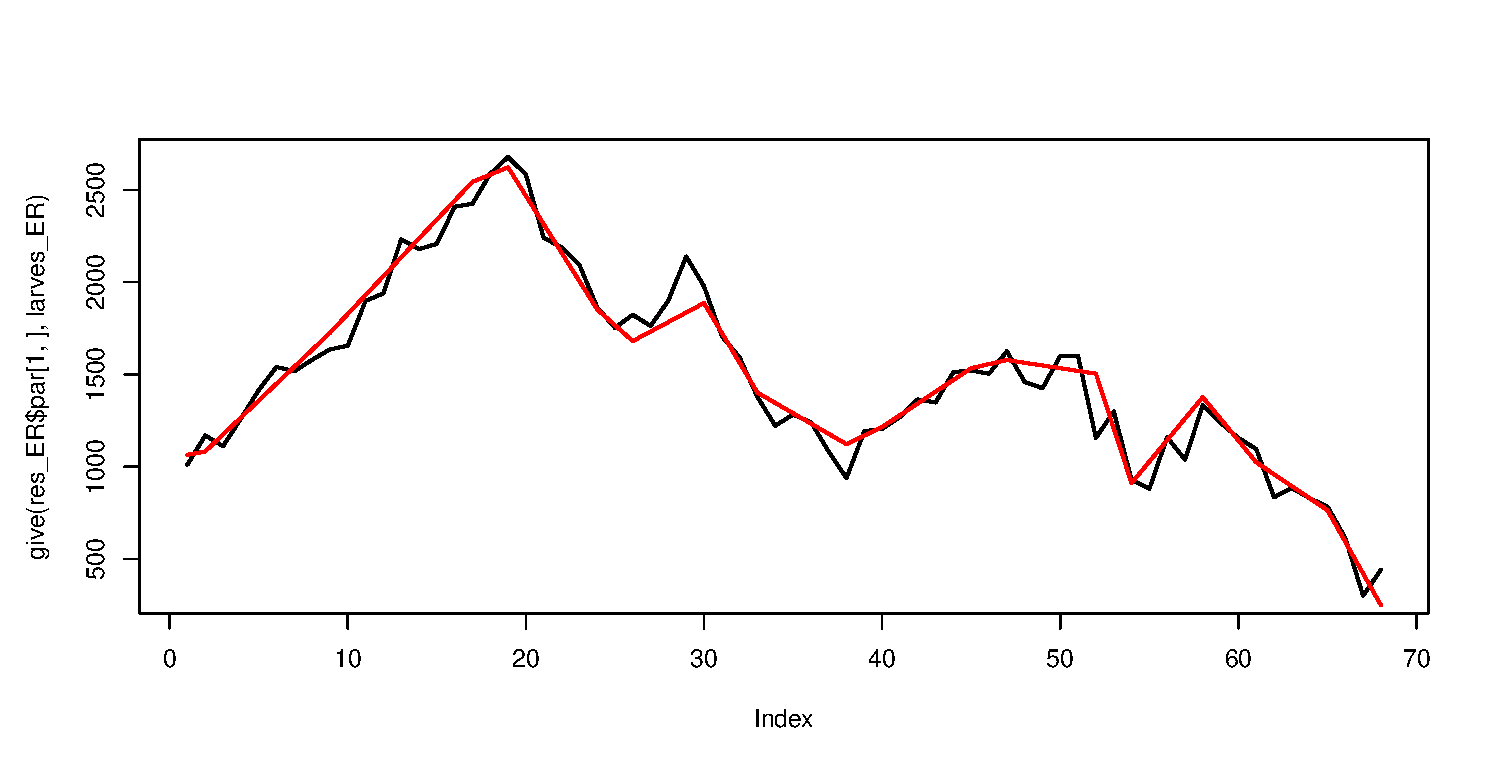
\epsfig{file = plots/cecido_ER.eps, scale = 0.65}
 \caption{}
\end{figure}

\newpage
\subsection{Paillage synthétique}

Les résultats sont les suivants :
\begin{verbatim}
alpha =

R =
mu =
E =
\end{verbatim}

\begin{figure}[ht]
 \centering
 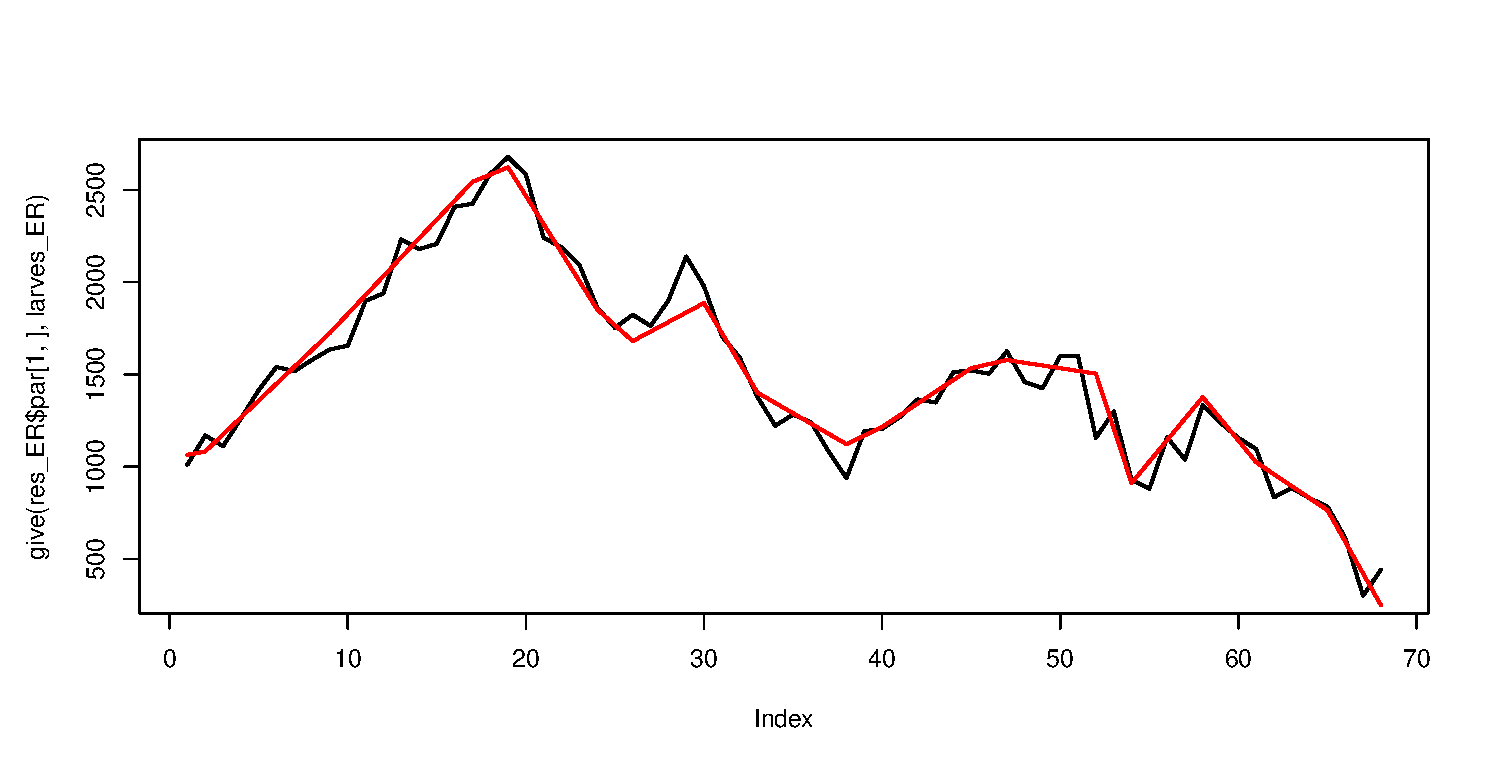
\epsfig{file = plots/cecido_ER.eps, scale = 0.65}
 \caption{}
\end{figure}

\newpage
\subsection{Enherbement haut}
\begin{verbatim}
alpha =

R =
mu =
E =
\end{verbatim}

\begin{figure}[ht]
 \centering
 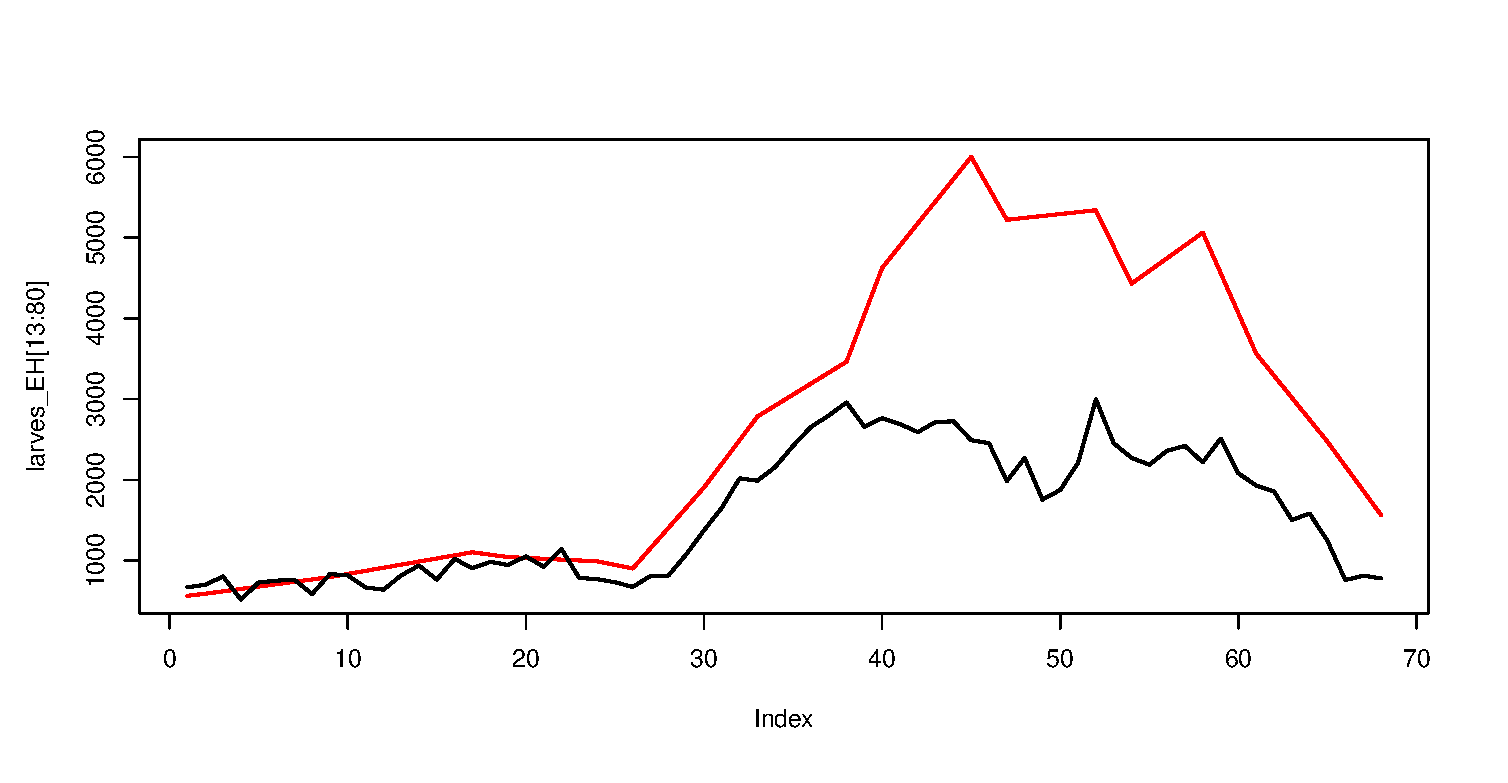
\epsfig{file = plots/cecido_EH.eps, scale = 0.65}
 \caption{}
\end{figure}





\end{document}
